\section{Rerigging Vrtnarija}


An early morning on expedition\ldots{} I stumble my way down to the
Bivi, late as ever, and set about fixing some coffee. It's a disturbing
hive of activity. William and James KP are planning to rig as far as
possible, replacing the rope below \passage{Pico} with new and rebolting
where necessary, Tetley is following them down and introducing the new
cavers to \passage{Vrtnarija}.

Excellent! Everything is in hand. Gergely suggests we follow up the rear
with extra rope and rigging gear, preparing the ground for tomorrow's
deep pushing. Looking forward to a nice, relaxing, afternoon trip, I
don't bother to cram food into myself (I'm never that innately hungry in
the mornings), and Gergely and I take the minimum of provisions.

It's nice to be back in \passage{Vrtnarija} again, after a year, and even
the stepping aside on the pitches to allow the vast quantities of cavers
to pass is fine. Eventually we pass everyone else \& get to \passage{Swing}, and
find William and James KP. They're both pretty pissed off: putting a new
bolt in on \passage{Swing} and rigging the blasted thing has sapped their energy.


\begin{pagefigure}
\checkoddpage \ifoddpage \forcerectofloat \else \forceversofloat \fi
   \centering
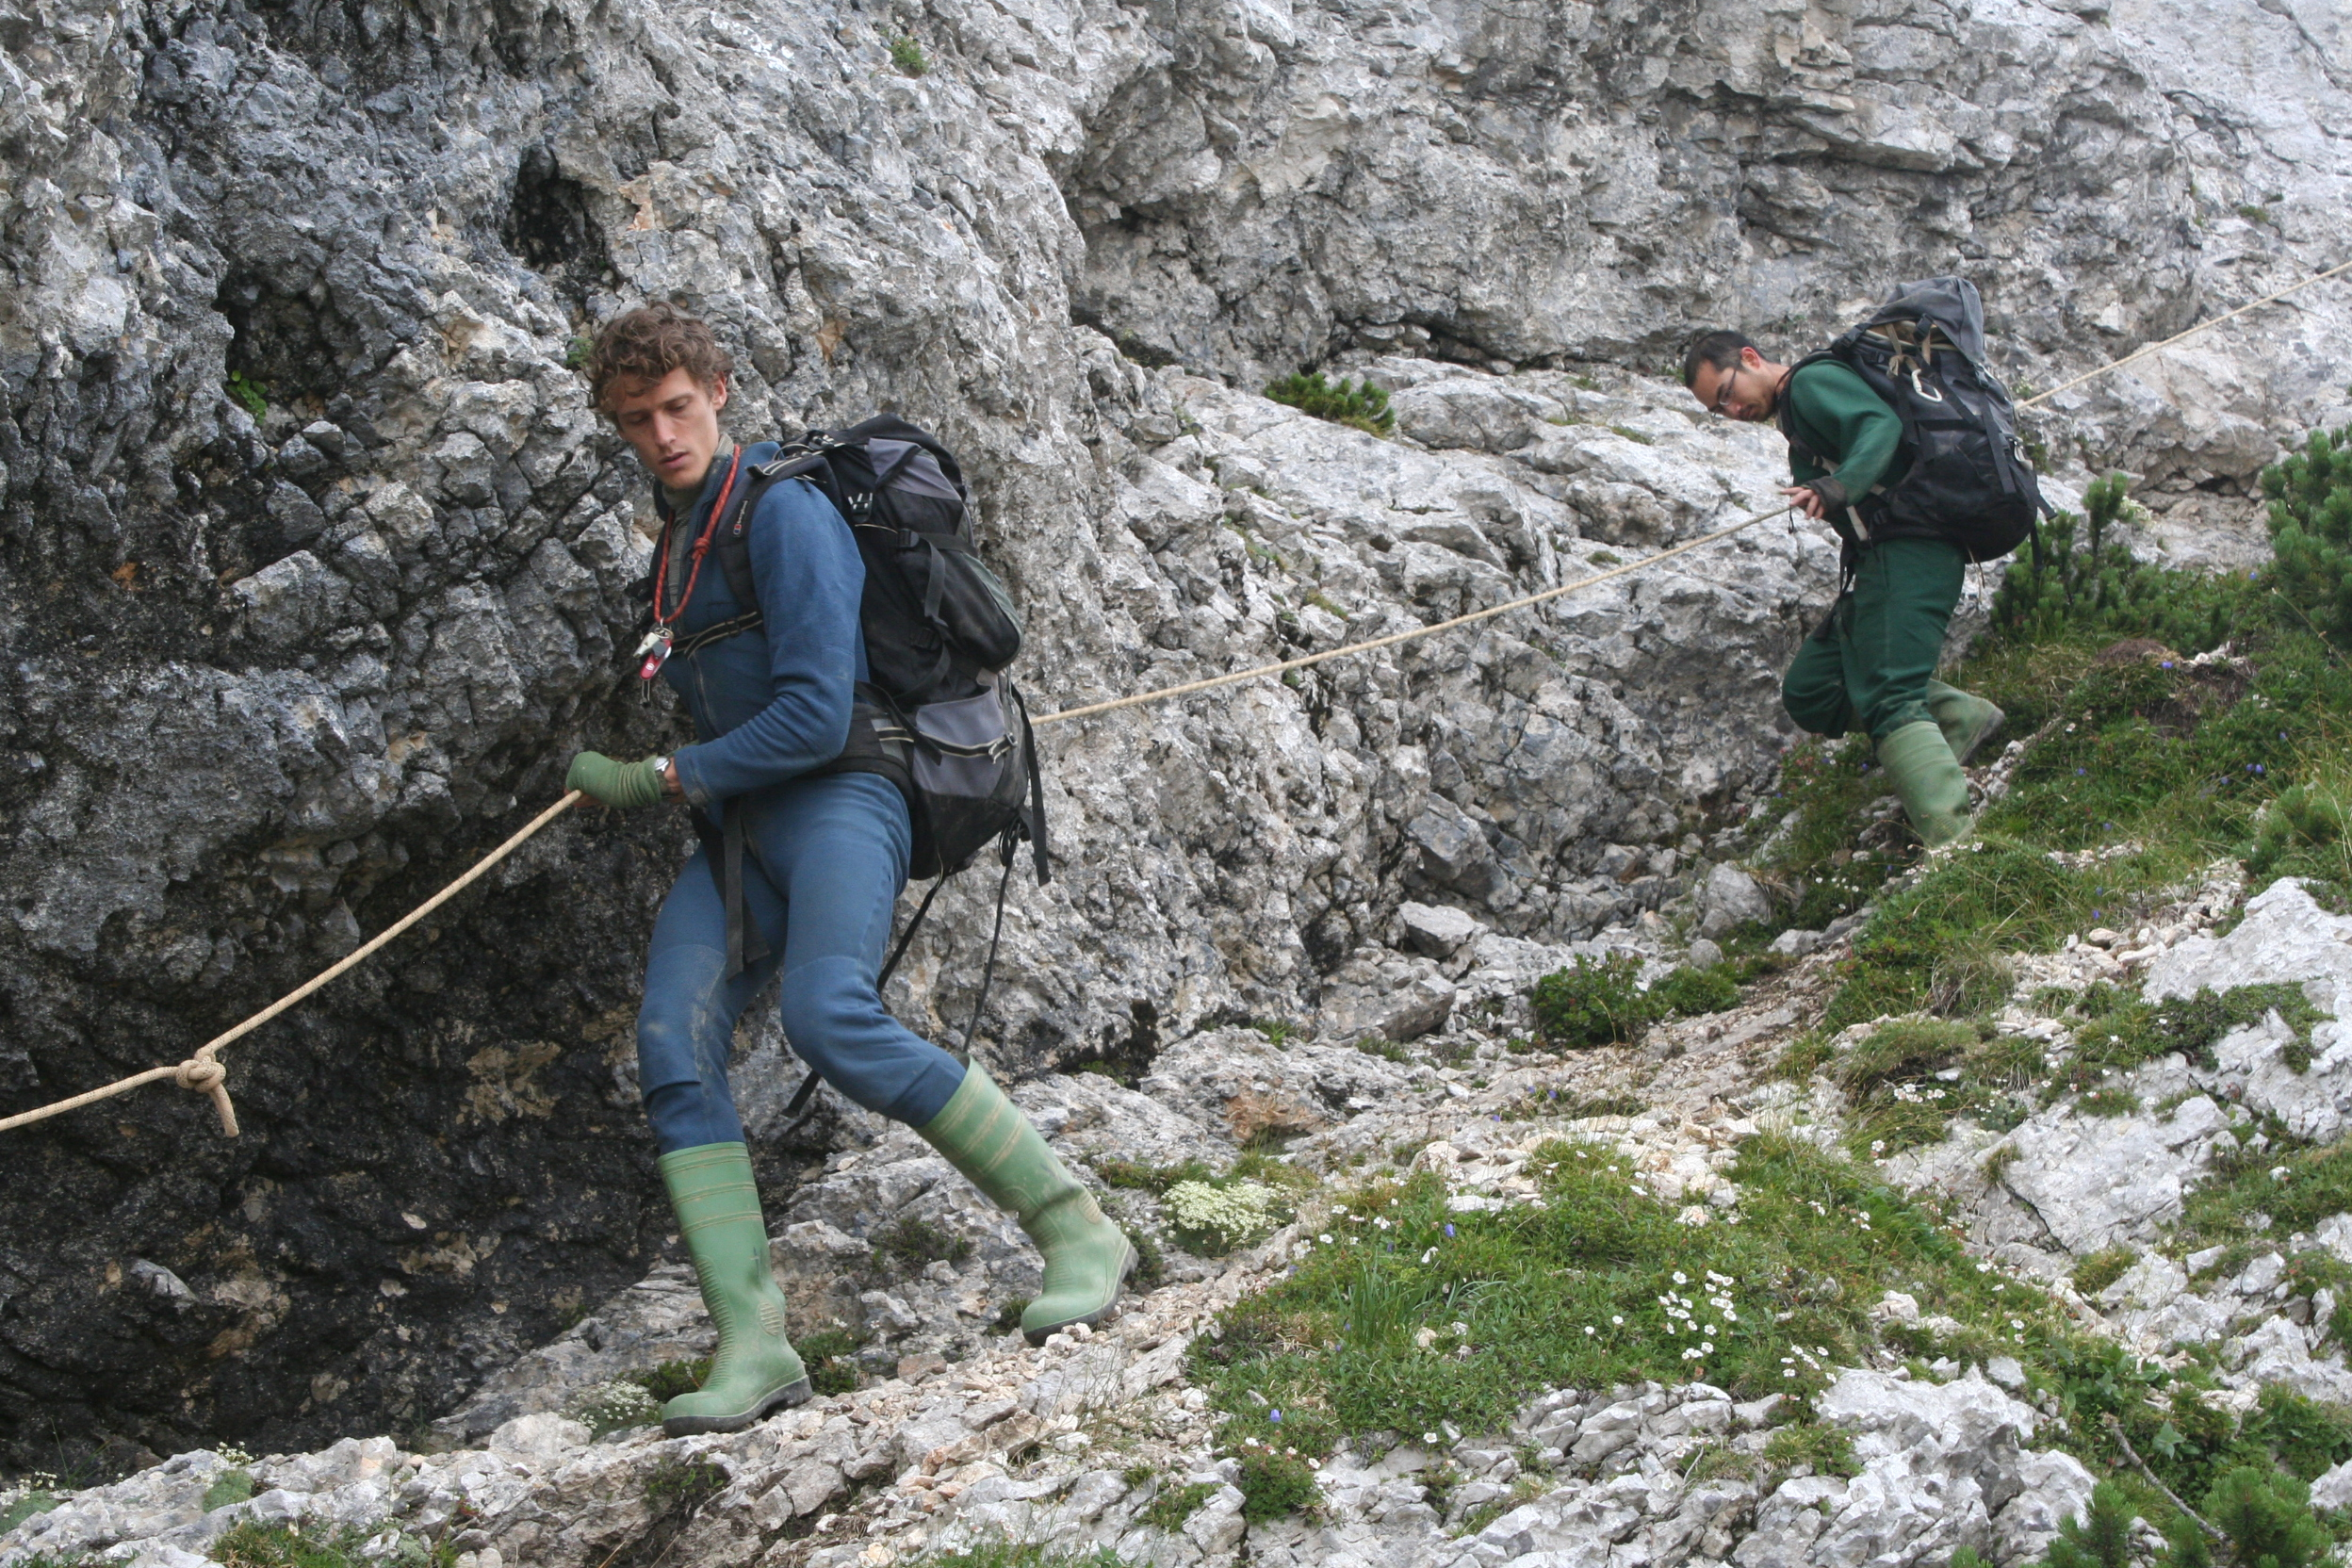
\includegraphics[width = \textwidth]{2010/expo_stories/20100810-11-17-37 - Jana Carga 35--orig.jpg}
\caption{On their way underground, Jarv and Thara use the handline rigged for assistance for the walk to/from \protect\passage{Vrtnarija}. \pic{Jana Čarga}} \label{handline to GW}
\end{pagefigure}


So Gergely and I take over. I rerig \passage{Tessellator}, coiling the old rope
ready for recovery. The head of \passage{space odyssey} receives an extra bolt and
thus a Y-hang - originally I intend to remove the deviation entirely, but find that I've misjudged slightly and it's still required, just.


\tweet{11:04PM Jul 20th, 2010}{10 cavers, 260m new rope, 3 bolt kits, 5 UG camp tackle sacks. VRTNARIJA rerigged to -300m, top of CONCORD. Great trips, cave is lovely.Jarv}


The traverse ledge halfway down \passage{space odyssey} needs more work. Gergely
comes down and we work on it together, me putting in more bolts and working new rope out along the traverse, whereas Gergely carefully
walked out on the old traverse and rigged the pitch down to \passage{Concorde}. We have a bit of confusion in the middle, as we also have to start a new rope. All sorted out, we have a spare 15 m of traverse rope that we hide for future use in a cubby hole.

Leaving the bolting kit and rope for future riggers, we have a smooth exit. Rather deeper and more effort than I had been intending for this first day's trip, and I was certainly feeling the lack of food as I prussic'ed back up the entrance series, but successfully completed nonetheless. In their first day of caving the expedition had rerigged down to -300 m!

\name{Jarvist Moore Frost}


\begin{figure*}
\checkoddpage \ifoddpage \forcerectofloat \else \forceversofloat \fi
\centering
    \begin{subfigure}{0.49\textwidth}
        \centering
        \frame{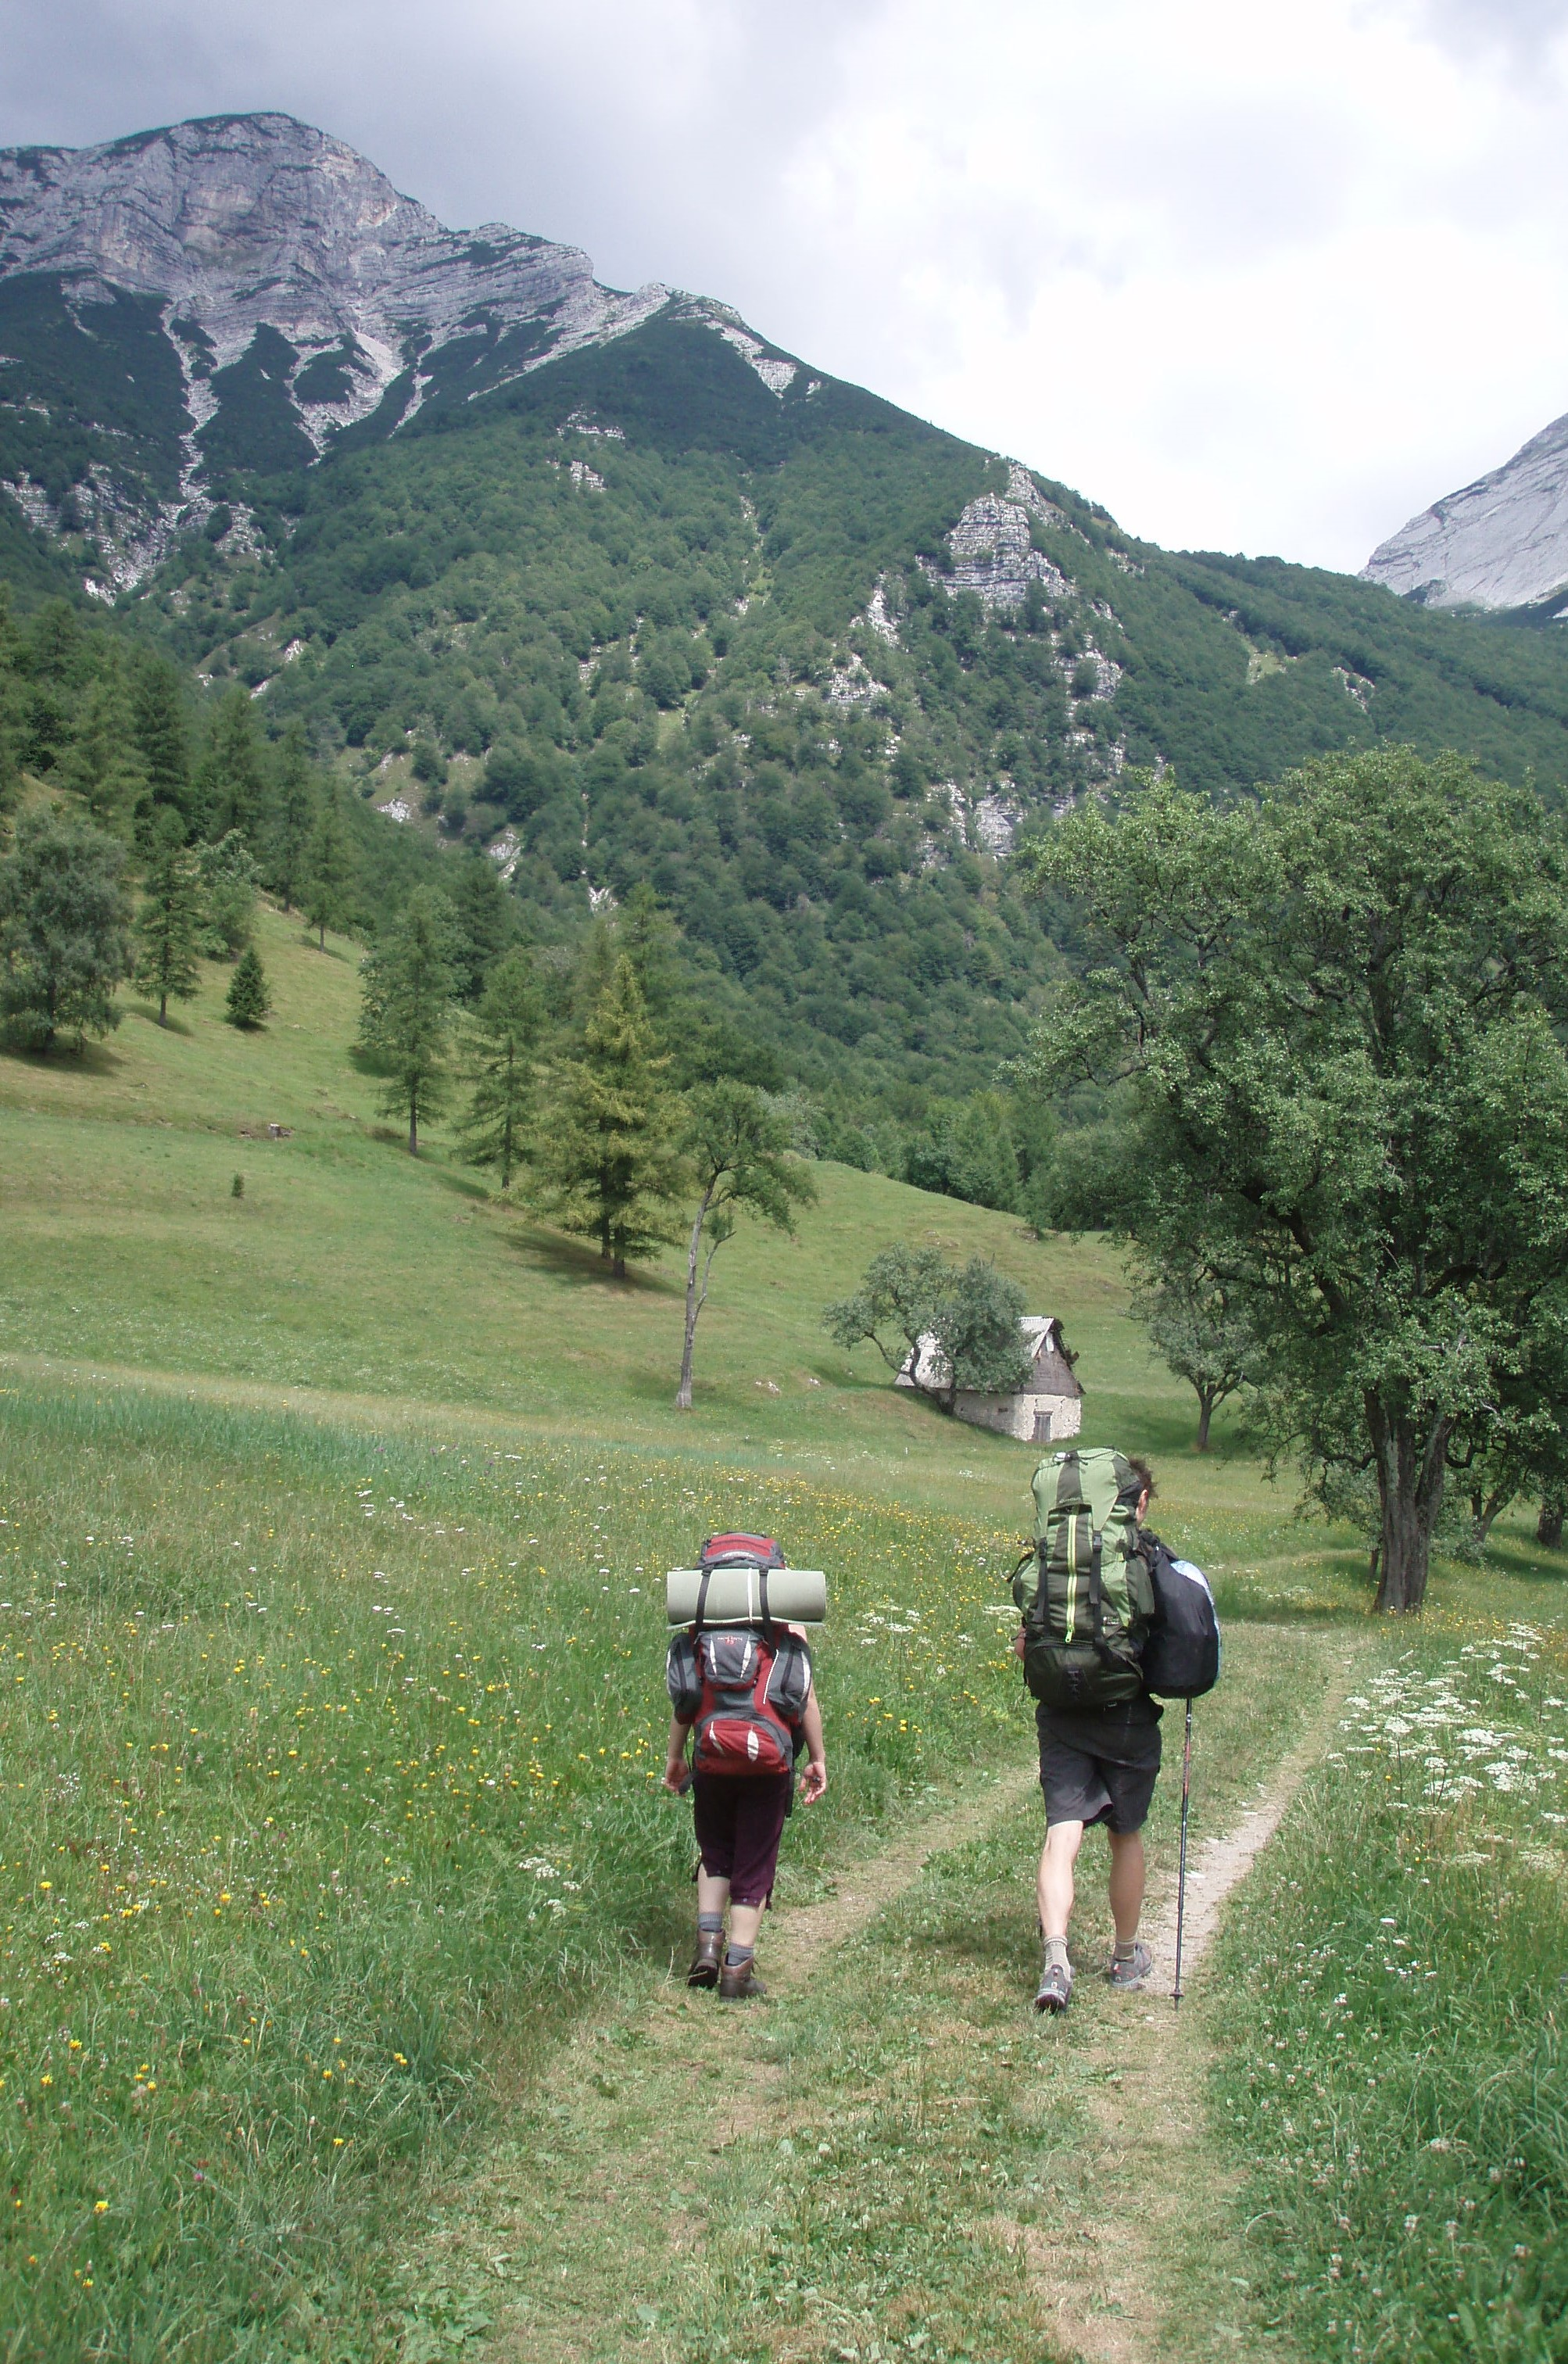
\includegraphics[width=\linewidth]{2010/expo_stories/20100803-22-02-59 - Jan Evetts - P2030068 - Ravne--orig.jpg}} 
        \caption{} \label{carries 2010}
    \end{subfigure}
        \hfill
\begin{subfigure}{0.49\textwidth}
\centering
\frame{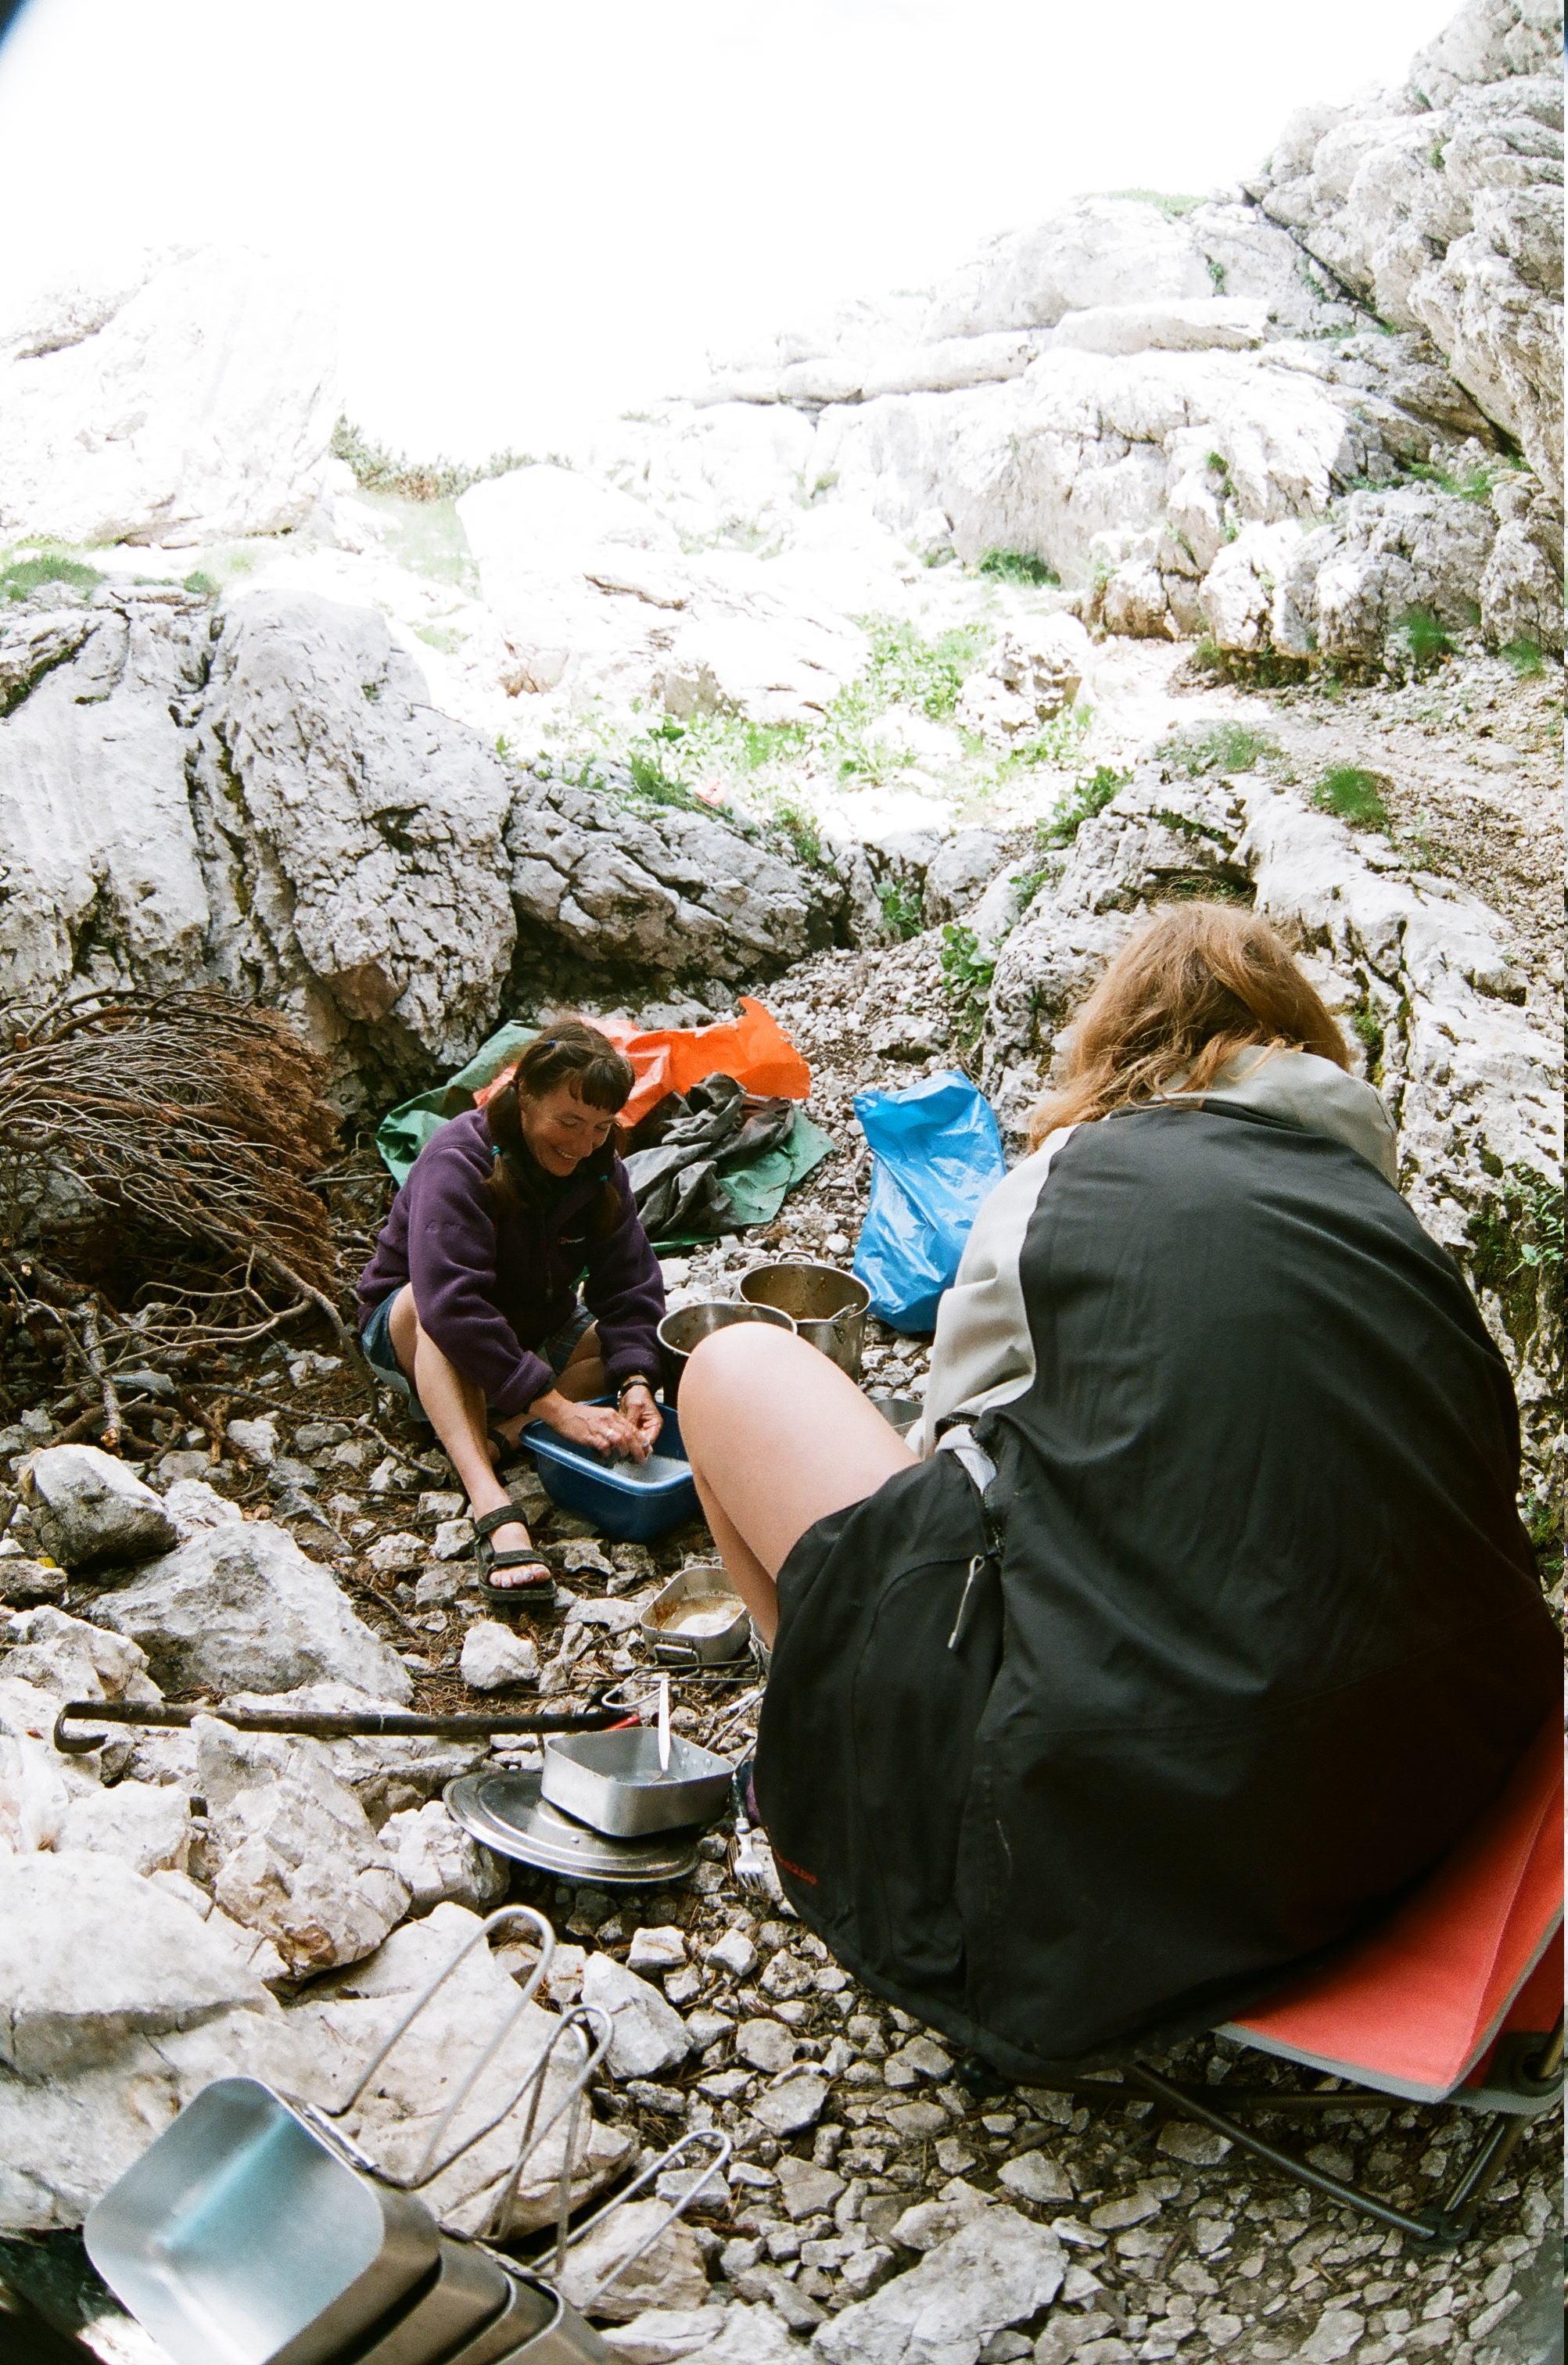
\includegraphics[width=\linewidth]{2010/expo_stories/Jarvist Frost - Canon A1 Zenit 16mm - 61320017--orig.jpg}}
 \caption{}\label{washing up}
\end{subfigure}
  \caption{\textit{a}) Setting off on a carry up the mountain. \pic {Jan Evetts} \textit{b}) Janet and Kate tackling the washing up, probably everybody's least favourite bivi task. \pic{Jarvist Frost}}
\end{figure*}